%Beamer class
\documentclass{beamer}

\usepackage[czech]{babel}
\usepackage[cp1250]{inputenc}
\usepackage{fontenc}
\usepackage{tgheros}
\usepackage{array}
\usepackage{color}
\usepackage{hyperref}

\usetheme{Antibes}
\usecolortheme{crane}


\title[BE1M13VES]{BE1M13VES}
\subtitle[Manufacturing of Electrical Components] {Manufacturing of Electrical Components}
\author[Brejcha]{Michal Brejcha}
\institute[CTU]{CTU in Prague}
\date[Prague, 2017]{Prague, 2017}

\begin{document}
%------------------------------------------------------------------------------
%Uvodni slajd
%------------------------------------------------------------------------------
\frame{\titlepage}

\begin{frame}
\frametitle{Overview} 
\tableofcontents
\end{frame}

\AtBeginSection[]
{
  \begin{frame}
    \frametitle{TOPIC}
    \tableofcontents[currentsection]
  \end{frame}
}

%------------------------------------------------------------------------------
%Capacitance
%------------------------------------------------------------------------------
\section{\texorpdfstring{Capacitance}{Capacitance}}
%------------------------------------------------------------------------------
	\begin{frame}
    \frametitle{Capacitors}
		\begin{tabular}{p{0.3\linewidth} p{0.6\linewidth}}
		\textbf{Parameters:} &
		\begin{itemize}
			\item $C$... capacitance
			\item $\delta$... tolearance
			\item $U$... nominal voltage
			\item $D$... dissipation factor 
			\item $ESR$... equivalent series resistance
			\item $TCC$... temperature coeficient of capacitance
			\item $VCC$... voltage coeficient of capacitance
			\item frequency dependence
		\end{itemize}
		\end{tabular}
  \end{frame}
%------------------------------------------------------------------------------
	\begin{frame}
    \frametitle{Capacitance of Capacitors}
		\begin{tabular}{p{0.3\linewidth} p{0.6\linewidth}}
		\textbf{Capacitance:} & $$C= \epsilon_0 \cdot \epsilon_r \cdot \frac{S}{d}$$
		\end{tabular}
		
		\begin{itemize}
			\item $\epsilon_0$ ... is the electric constant ($\epsilon_0\approx 8.854 \cdot 10^{-12}$ F/m),
			\item $\epsilon_r$ ... is the relative static permittivity,
			\item $S$ ... is the area of overlap of the two plates,
			\item $d$ ... is the separation between the plates.
		\end{itemize}
		\begin{center}
			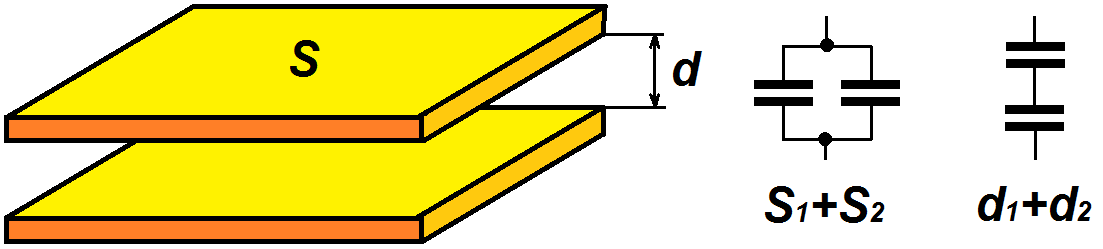
\includegraphics[scale=0.3]{obr01_kapacita.png}
		\end{center}
  \end{frame}
%------------------------------------------------------------------------------
%Technology
%------------------------------------------------------------------------------
\section{\texorpdfstring{Technology}{Technology}}
%------------------------------------------------------------------------------
	\begin{frame}
    \frametitle{Technology Overview}
		Technologies are derived from dielectric material:
		
		\begin{itemize}
			\item Air, vacuum capacitors
			\item Ceramic capacitors (NP0, X5R,...)
			\item Film (foil) capacitors (paper, PP,...)
			\item Electrolytic capacitors (Al$_2$O$_3$,...)
		\end{itemize}
		\begin{center}
			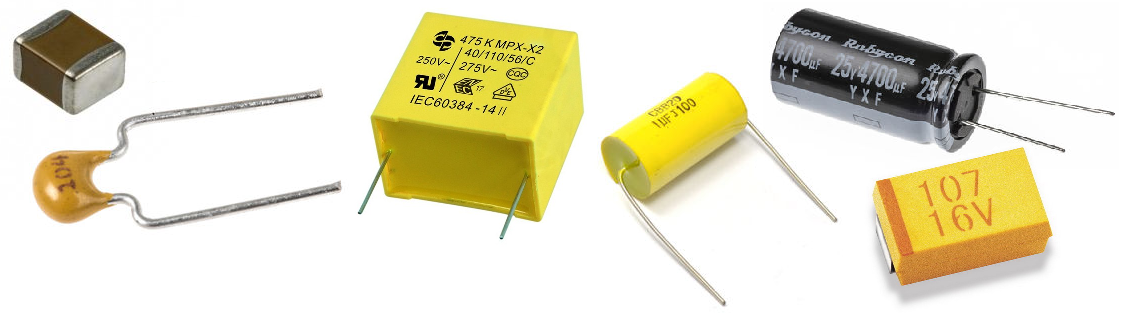
\includegraphics[scale=0.35]{obr02_kondenzatory.png}
		\end{center}
  \end{frame}
%------------------------------------------------------------------------------
	\begin{frame}
    \frametitle{Vacuum Capacitor}
		\begin{center}
			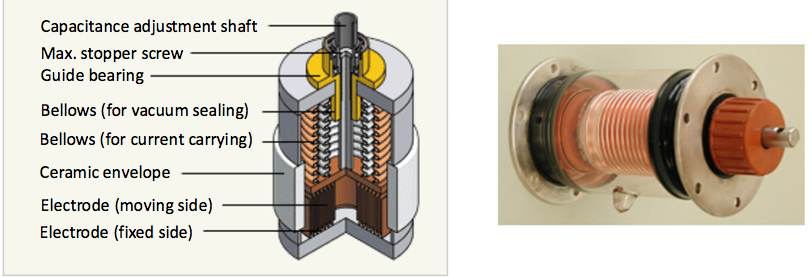
\includegraphics[scale=0.38]{obr03_vakuovyKond.png}\\
			
			\tiny{\textbf{Source:}~renosubsystems.com/plasma-etching-deposition-technologies/rf-matching-networks/}
		\end{center}
		\small
		
		\begin{itemize}
			\item Electrodes (stator and rotor) are very similar to air capacitors.
			\item Advantageous is higher insulation capability. Maximum applied voltage is given just by auto-emission of electrons between stator and rotor parts.
			\item Most widespread design is vacuum tube similar to electron tubes.  Most critical is hermetic sealing (glass tubes).
			\item Low power dissipation.
		\end{itemize}
  \end{frame}
%------------------------------------------------------------------------------
	\begin{frame}
    \frametitle{Air Capacitor}
		\small
		\begin{tabular}{m{0.45\linewidth} m{0.45\linewidth}}
		\begin{itemize}
			\item They are created with a set of metal plates separated with an air dielectric.
			\item Power losses are negligible.
		\end{itemize}
		& 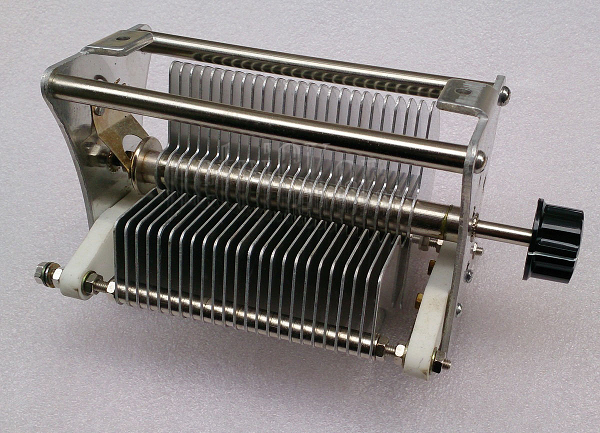
\includegraphics[scale=0.3]{obr04_vzduchovyKond.png}
		\end{tabular}
		\begin{tabular}{m{0.9\linewidth}}
		\begin{itemize}
			\item They are used as tuning and variable capacitors.
			\item Maximum applied voltage is given just with the air-isolation capability.
		\end{itemize}
		\end{tabular}
  \end{frame}
%------------------------------------------------------------------------------
	\begin{frame}
    \frametitle{Foil Capacitors}
		\begin{center}
			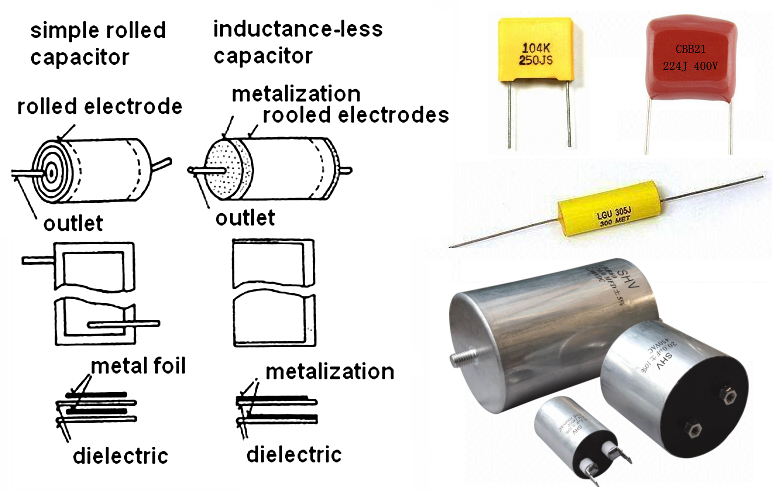
\includegraphics[scale=0.5]{obr05_foliovyKond.png}
		\end{center}
  \end{frame}
%------------------------------------------------------------------------------
	\begin{frame}
    \frametitle{Foil Capacitors}
		\small
		\begin{description}
		\item[\textbf{dielectric}] dry paper for capacitors (natron-celluloze) from 6 to 20 $\mu m$ thickness, typically 2 layers. Plastic foils: polystyrene, polyethylentherepthalath (PETP), polycarbonate, polyimide, polypropylene,
		\item[\textbf{electrodes}] aluminum foil, thickness - units of $\mu m$,
		\item[\textbf{leads}] copper pads bonded directly on electrodes, copper wires rolled into bulk of capacitor.
		\end{description}
		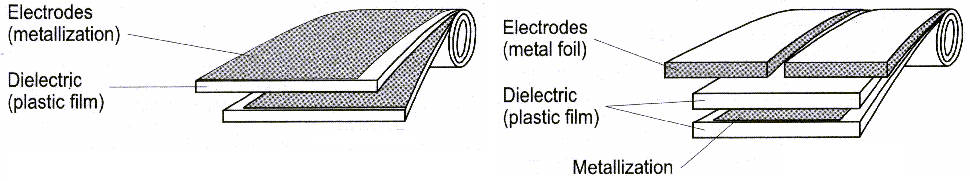
\includegraphics[scale=0.4]{obr06_navijeni.png}
  \end{frame}
%------------------------------------------------------------------------------
	\begin{frame}
    \frametitle{Arrangement for high voltage}
		\begin{center}
			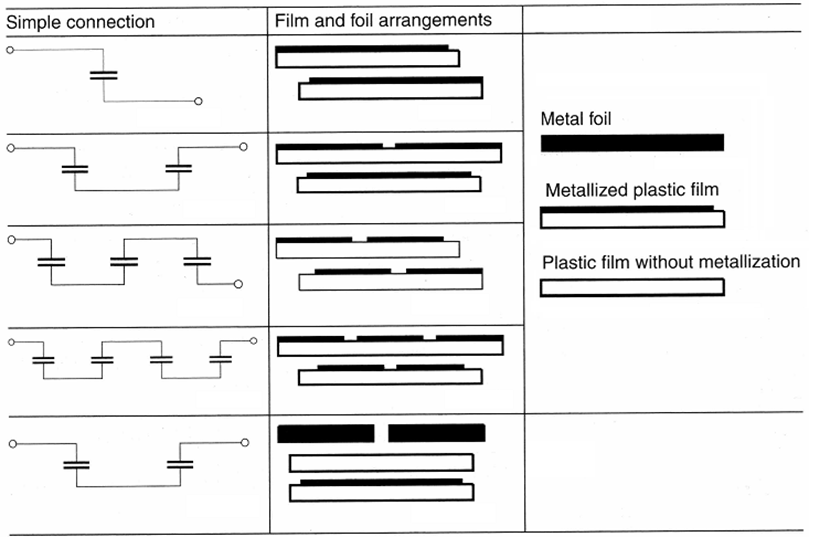
\includegraphics[scale=0.45]{obr07_usporadani.png}
		\end{center}
  \end{frame}
%------------------------------------------------------------------------------
	\begin{frame}
    \frametitle{Ceramic Capacitors}
		Ceramic material with relative permittivity from range $1$ (linear) up to $10^4$ (ferroelectric) is used for dielectric layer. Conductive surface of electrodes is made from silver. Silver is deposited by evaporation.
		
		\begin{itemize}
			\item \textbf{the oldest ceramics (1930):} were based on oxides of titan and manganum \\($\epsilon_r=10-100$, TCC from $-750$ to $100\cdot 10^{-6}$ $^\circ$C$^{-1}$).
			\item \textbf{titan based ceramics:} ($BaTiO_3$, $CaTiO_3$, $SrTiO_3$, $MgTiO_3$) have $\epsilon_r$ in range 1000 - 20000 but they are ferroelectric - exhibit Curie's temperature, dielectric hysteresis and they are voltage dependent.
		\end{itemize}
  \end{frame}
%------------------------------------------------------------------------------
	\begin{frame}
    \frametitle{Ceramic Capacitors - Types}
		\textbf{capacitor called \uv{class 1}: }
		\begin{itemize}
			\item stable and linear $\epsilon_r$,
			\item low power loss: D factor at maximum $2\cdot 10^{-3}$,
			\item TCC from $-680$ to $200\cdot 10^{-6}$ $^\circ$C$^{-1}$,
			\item voltage independent.
		\end{itemize}
		\small
		\textbf{Commercial names:} \\STEALIT (similar to porcelain), STABILIT, TEMPA, RUTILIT, KONDENSA, NEGALIT. \\Typically contain $TiO_2$, $MgO$, $ZrO_2$. Such capacitors are good for high frequency and high voltage applications.

  \end{frame}
%------------------------------------------------------------------------------
	\begin{frame}
    \frametitle{Ceramic Capacitors - Types}
		\textbf{capacitor called \uv{class 2}: }
		\begin{itemize}
			\item dielectric with high $\epsilon_r$,
			\item ferroelectric features (voltage dependent),
			\item very temperature sensitive. Peak of maximum $\epsilon_r$ can be shifted by additional oxides ($SrTiO_3$, $PbTiO_3$, $BaSnO_3$, $CaSnO_3$) or flatten ($CaTiO_3$, $Bi_2SnO_3$).
		\end{itemize}
		\small
		\textbf{Commercial names:} \\PERMITIT ($BaTiO3$, $D$ max. $3\cdot10^{-2}$, tolerance $\pm 50 \%$). Suitable for coupling and filtering capacitors.
		\begin{center}
			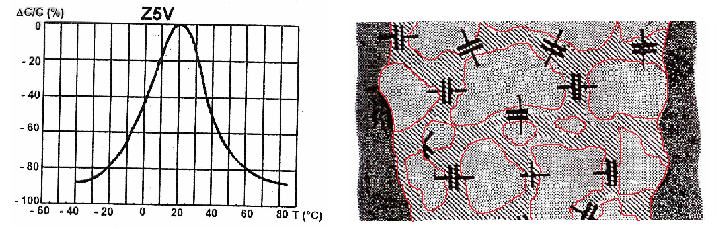
\includegraphics[scale=0.45]{obr08_feroelektrikum.png}
		\end{center}
  \end{frame}
%------------------------------------------------------------------------------
	\begin{frame}
    \frametitle{Ceramic Capacitors - Types}
		\textbf{capacitor called \uv{class 3}: }
		\begin{itemize}
			\item dielectric with high $\epsilon_r$,
			\item similar ceramic as for \uv{class~2} but different burning process (re-oxide ceramic),
			\item large power loss, due to high electrical strength in ferroelectric, ceramic exhibit some \uv{semiconductor} behavior,
			\item Material has a domain structure - ferroelectric properties again. 
		\end{itemize}
		\small
		\textbf{Commercial names:} \\SUPERMIT, SIBATIT ($\epsilon_r$ approximately $5\cdot 10^4$).\\These capacitors are not high-quality devices, ideal for low-cost application.

  \end{frame}
%------------------------------------------------------------------------------
	\begin{frame}
    \frametitle{Mechanical Design - SMD}
		\begin{center}
			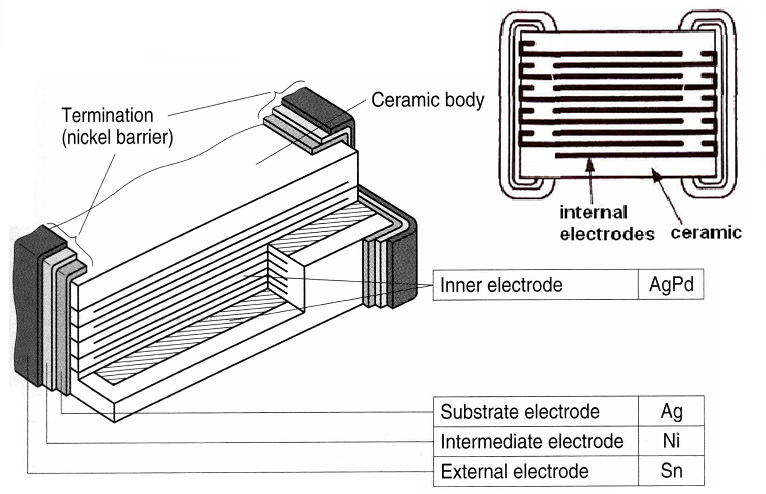
\includegraphics[scale=0.45]{obr09_smdKonstrukce.png}
		\end{center}
  \end{frame}
%------------------------------------------------------------------------------
	\begin{frame}
    \frametitle{Electrolytic Capacitor}
		\small
		\begin{tabular}{m{0.55\linewidth}m{0.35\linewidth}}
		\begin{flushleft}
		\textbf{Dielectric:} created by a very thin oxide layer placed on one side of electrode. Thickness allows to achieve large capacity in a small volume. Disadvantageous is a polarization of oxide layer.
		\end{flushleft}
		\begin{flushleft}
		\textbf{Design:} aluminum electrolytic capacitors are similar to rolled capacitors. Rolled electrodes are made of aluminum strip. Surface is enlarged by brushing and finally is etched. Dielectric layer is formed by anodic oxidation process. Rolled strips are impregnated by electrolyte.
		\end{flushleft}
		& 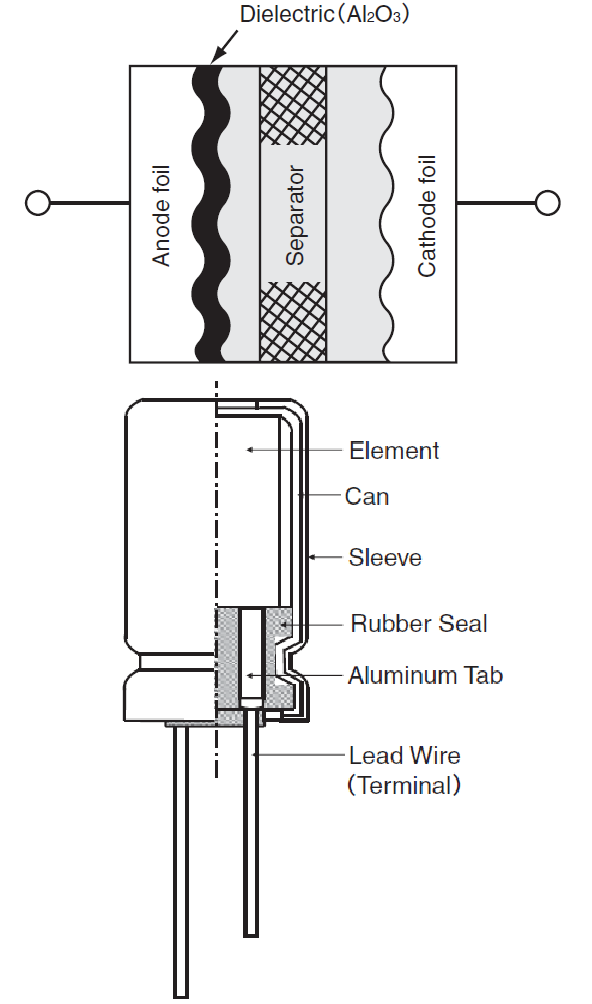
\includegraphics[scale=0.25]{obr12_elektrolyt.png}
		\end{tabular}
  \end{frame}
%------------------------------------------------------------------------------
	\begin{frame}
    \frametitle{Features}
		\begin{tabular}{m{0.6\linewidth} m{0.3\linewidth}}
		\begin{itemize}
			\item High capacity due to small insulation thickness and large surface,
			\item only one polarity,
			\item relatively small maximum nominal voltage:
			
			\begin{itemize}
				\item Aluminum (Al$_2$O$_3$) up to 500~V
				\item Tantalum (Ta$_2$O$_5$) up to approximately 50~V (100~V)
			\end{itemize}
		\end{itemize} & 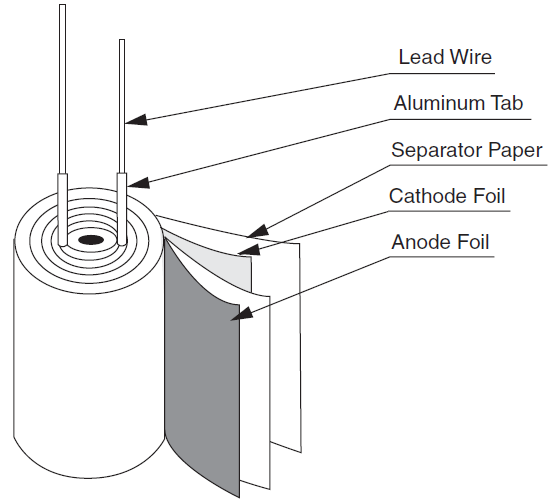
\includegraphics[scale=0.25]{obr14_elektrolytKonst.png}
		\end{tabular}
		\textbf{Aluminum Electrolytic Capacitors:}
		\begin{flushleft}
		They have similar design to foil capacitors. Anode and Cathode is made of Aluminum. Part of the cathode is made by electrolyte (acid $H_3BO_3$).
		\end{flushleft}
  \end{frame}
%------------------------------------------------------------------------------
	\begin{frame}
    \frametitle{Tantalum Electrolytic Capacitors}
		\begin{tabular}{m{0.3\linewidth} m{0.6\linewidth}}
		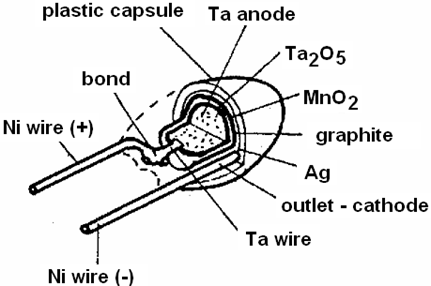
\includegraphics[scale=0.35]{obr15_tantalum.png} &
		\begin{itemize}
			\item Higher capacity due to very small insulation thickness
			\item Better ESR - Equivalent Serial Resistance
			\item Smaller breakdown voltages
		\end{itemize}
		\end{tabular}
		\textbf{Anode:} Made from burned Ta powder, then oxidized in $H_3PO_4$
		\begin{flushleft}
		\textbf{Cathode:} Capacitors with liquid electrolyte have hermetic Ag capsules (cathode). Acid $H_2SO_4$ is used as electrolyte. Capacitors with solid electrolyte don't have hermetical capsule, $MnO_2$ is used as electrolyte, cathode is made from colloidal graphite and silver.
		\end{flushleft}

  \end{frame}
%------------------------------------------------------------------------------
%Parasitic Parameters
%------------------------------------------------------------------------------
\section{\texorpdfstring{Parasitic Parameters}{Parasitic Parameters}}
%------------------------------------------------------------------------------
	\begin{frame}
    \frametitle{Power Dissipation Factor}
		\begin{center}
		\small
		\begin{tabular}{m{0.4\linewidth} m{0.5\linewidth}}
		$$D=tg\delta=\frac{P_{loss}}{Q}=...$$
		For parallel scheme (figure)
		$$...=\frac{I_R}{I_C}= \frac{1}{\omega CR}$$
		& 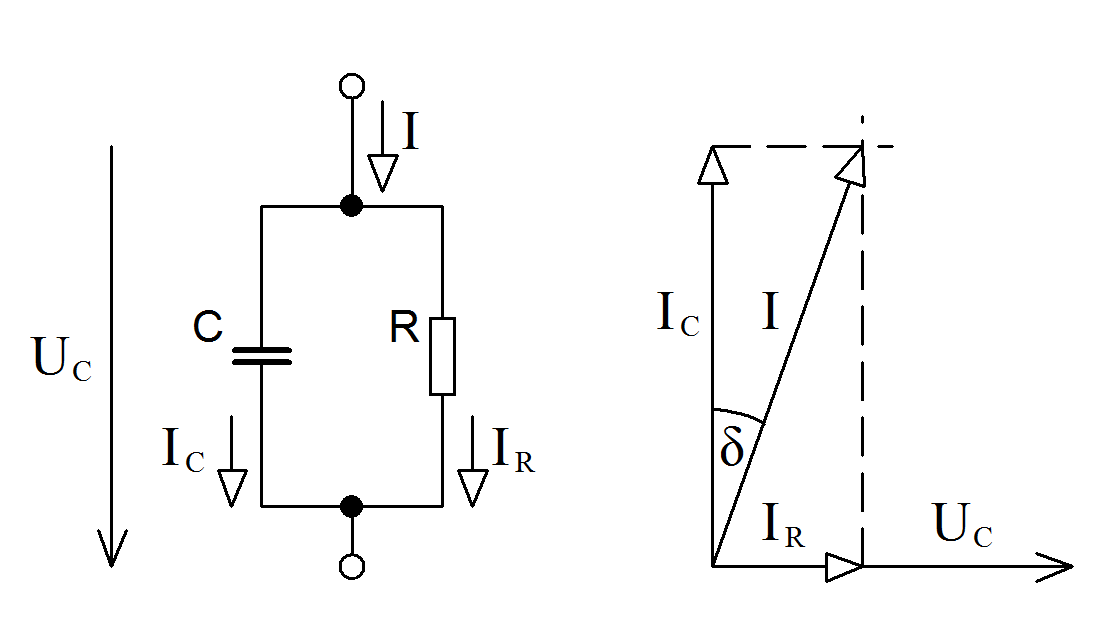
\includegraphics[scale=0.2]{obr16_tgDelta.png}
		\end{tabular}
		\end{center}
		\begin{flushleft}
			\textbf{Dissipation factor} describes the total power losses in dielectric at AC supply. Dissipation factor includes all losses in dielectric material and ohmic losses in wire outlets and electrodes.
		\end{flushleft}
  \end{frame}
%------------------------------------------------------------------------------
	\begin{frame}
    \frametitle{Temperature and Voltage Dependency}
		\small
		\begin{itemize}
			\item Similar description as for resistors via TCC (Temperature Coefficient of Capacitance): $$C= C_0\cdot\left(1+TCC\cdot(T-T_0)\right)$$ and via VCC (Voltage Coefficient of Capacitance): $$C= C_0\cdot\left(1+VCC\cdot(T-T_0)\right)$$
			\item It can be considered linear in case of foil capacitor or ceramic capacitor of class 1. The TCC is very small.
			\item TCC is very high and dependent on temperature in case of ceramic capacitors of class 2 and 3.
			\item Quite strong dependency on temperature is also in case of aluminum electrolytic capacitors. Tantalum capacitors are voltage and temperature stable.
		\end{itemize}
  \end{frame}
%------------------------------------------------------------------------------
	\begin{frame}
    \frametitle{Temperature Dependency - Ceramic Capacitors}
		\begin{center}
			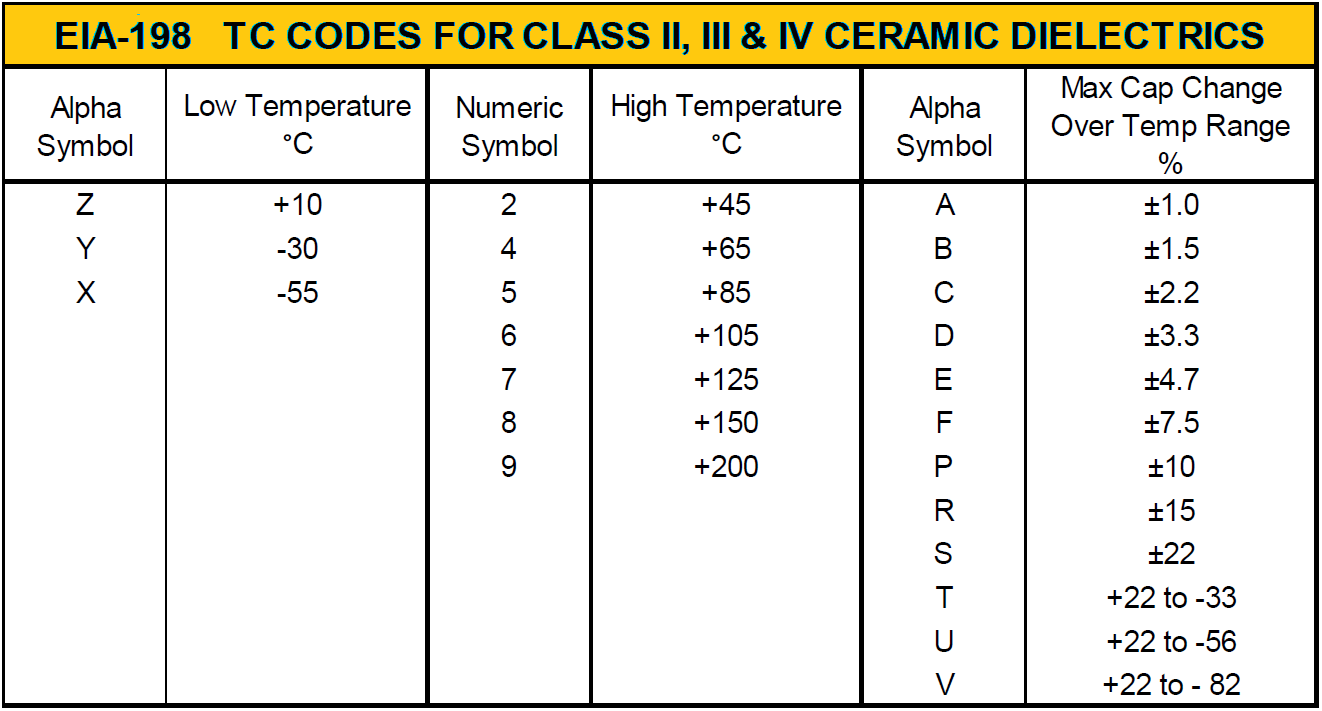
\includegraphics[scale=0.3]{obr13_kodovani.png}
		\end{center}
  \end{frame}
%------------------------------------------------------------------------------
	\begin{frame}
    \frametitle{Temperature Dependency - Ceramic Capacitors}
		\begin{center}
			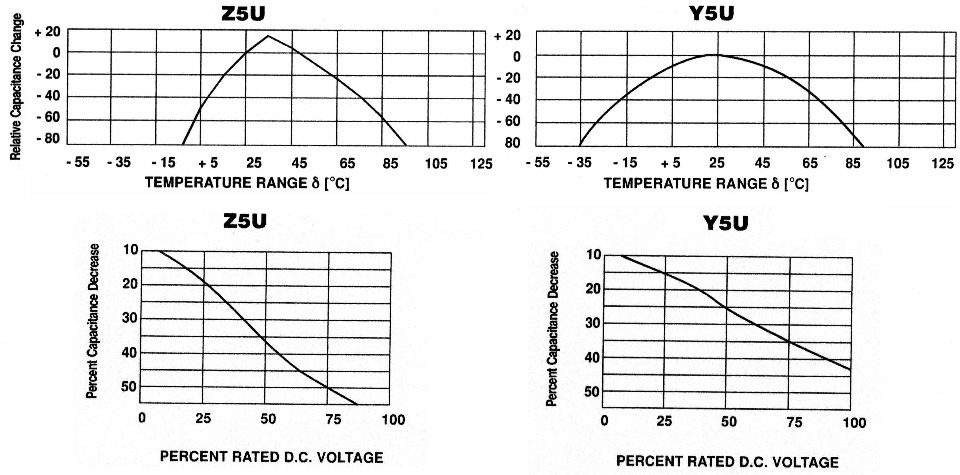
\includegraphics[scale=0.4]{obr10_tepZav.png}
		\end{center}
  \end{frame}
%------------------------------------------------------------------------------
	\begin{frame}
    \frametitle{Voltage Dependency - Ceramic Capacitors}
		\begin{center}
			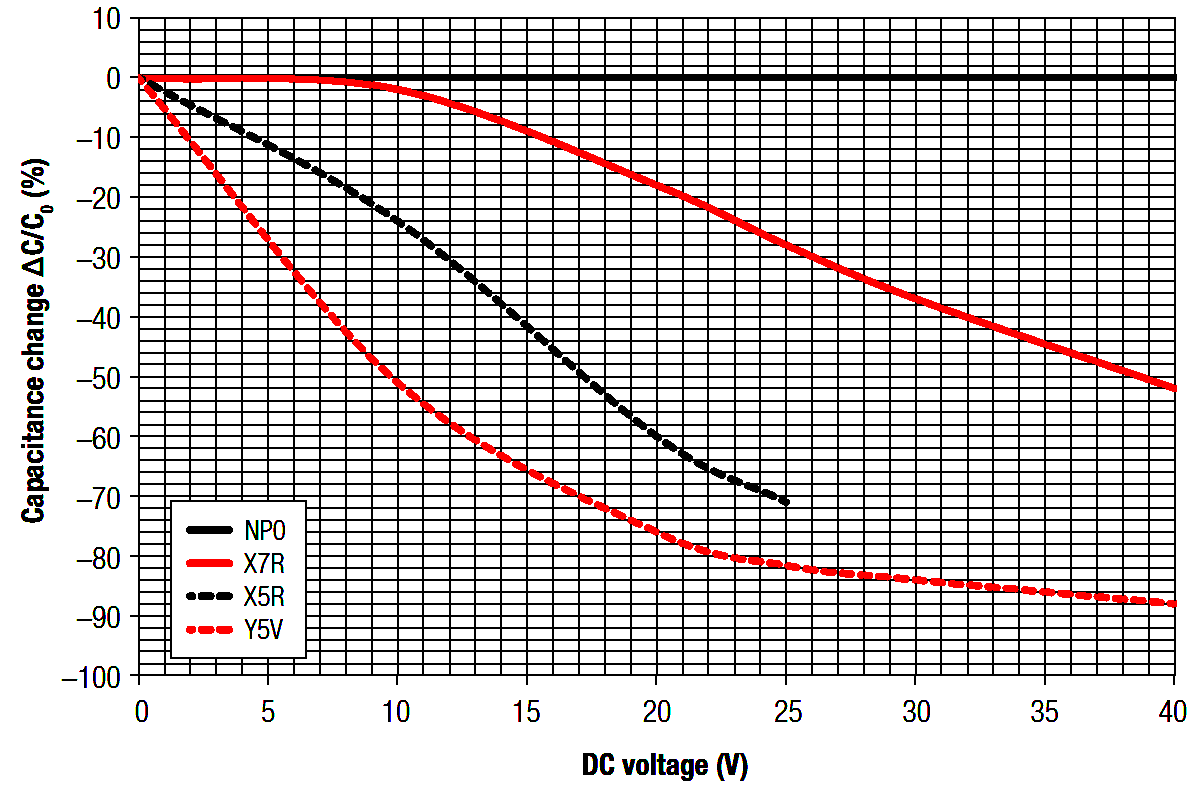
\includegraphics[scale=0.3]{obr11_napZav.png}
		\end{center}
  \end{frame}
%------------------------------------------------------------------------------
\end{document}